\section{Latency and Defragmentation Trade-off Test}
\label{sec:netaware4_test}
%-----------------------------------------------------------------------------%
In this section we evaluates the trade-off between network latency preservation and resource defragmentation within a Kubernetes cluster using the proposed Network-Aware plugin. The evaluation focuses on how the plugin maintains communication efficiency by preventing pod evictions that could potentially increase network latency. The experiments are conducted using three balancing strategies, namely LowNodeUtilization, HighNodeUtilization, and custom ResourceDefragmentation, to analyze the impact of network-aware eviction filtering under different workload redistribution approaches.

%-----------------------------------------------------------------------------%
\subsection{Experimental Setup and Environment Configuration}
\label{subsec:netaware4_experimentsetup}
%-----------------------------------------------------------------------------%
To evaluate the effectiveness of the proposed Network-Aware Descheduler against resource fragmentation and degraded latency anomalies, we built a physical-to-logical hybrid testing sandbox. The design validates descheduling actions against varying node performance tiers under tight resource ceilings, providing deterministic telemetry data for thesis synthesis.

%-----------------------------------------------------------------------------%
\subsubsection{Infrastructure and Cluster Topology}
\label{subsubsec:netaware4_infrasetup}
%-----------------------------------------------------------------------------%
The experimental testing cluster is hosted inside an isolated Virtual Private Cloud (VPC) on Amazon Web Services (AWS). Due to the structural restrictions of the cloud sandbox environment, all instances are physically provisioned within the \textit{us-east-1} geographic region. The infrastructure pool comprises five distinct \textit{t3.micro} virtual machines acting as worker nodes, alongside a dedicated administrative control plane and one worker specific for Prometheus.  

A critical engineering constraint of the \textit{t3.micro} hardware profile is its highly restricted footprint: each instance features 2 vCPUs and a bare 1 GiB (1024 MiB) of physical RAM. After accounting for vital system daemon overheads (including the Linux kernel, Kubelet, container runtime, and Flannel network plugins), the net allocatable memory per node drops to a constrained window of approximately 800 MiB.  

To model real-world high-availability environments, the underlying physical cluster nodes are distributed across distinct Availability Zones (AZs) as follows:  

\begin{itemize}
    \item \textit{us-east-1d}: worker-1, worker-2
    \item \textit{us-east-1b}: worker-3
    \item \textit{us-east-1a}: worker-4, worker-5
\end{itemize}

%-----------------------------------------------------------------------------%
\subsubsection{Network Profile and Topology Modeling}
\label{subsubsec:netaware4_networksetup}
%-----------------------------------------------------------------------------%
To evaluate the impact of network locality on scheduling and descheduling decisions, the cluster topology was configured to include nodes with heterogeneous network characteristics distributed across multiple logical availability zones:

\begin{itemize}
    \item \textbf{Normal Network Conditions:} Consists of worker-1, worker-2, and worker-3. These nodes retain their native cloud-provider network performance. Communication within the same availability zone experiences approximately 0.3 ms latency, while communication across availability zones incurs a natural latency of approximately 1-2 ms.

    \item \textbf{Degraded Network Conditions:} Consists of worker-4 and worker-5, which are assigned to a separate logical availability zone and configured to emulate constrained network conditions. These nodes experience significantly higher communication latency than the rest of the cluster, representing a lower-quality network domain within the topology.
\end{itemize}

To achieve the network degradation, the primary operating system network interface (\emph{ens5}) on both worker-4 and worker-5 was targeted. A deterministic outbound network emulation queue discipline (\emph{qdisc}) rule was applied directly to the root interface using the Linux Traffic Control (\emph{tc}) framework:

\begin{lstlisting}[language=bash, numbers=none, xleftmargin=0.5em, framexleftmargin=0em]
sudo tc qdisc add dev ens5 root netem delay 80ms 5ms distribution normal
\end{lstlisting}

Crucially, because this traffic shaping rule acts as a uniform egress filter, it creates a multi-hop latency matrix depending on the communication path. When a normal node (worker-1) initiates a round-trip connection with a degraded node (worker-4), the packet triggers an 80 ms delay leaving worker-4's interface during the response phase. However, when worker-4 and worker-5 communicate with each other, both machines enforce their outbound egress rules. This creates an additive round-trip time (RTT) accumulation:

\[
RTT_{\text{Tier2}\leftrightarrow\text{Tier2}} = Delay_{\text{Node4 (Egress)}} + Delay_{\text{Node5 (Egress)}} \approx 160\,\text{ms}
\]


%-----------------------------------------------------------------------------%
\subsubsection{Telemetry and Monitoring Architecture}
\label{subsubsec:netaware4_monitoringsetup}
%-----------------------------------------------------------------------------%
To provide the network-aware descheduler with continuous data streams, we deployed a tight telemetry loop combining a full-mesh prober with a time-series database.

Bloomberg's Goldpinger (version 3.10.1) was deployed as a cluster-wide DaemonSet, pinning a network auditing pod to each of the five worker nodes. Every 30 seconds, each Goldpinger instance executes a cross-node internal web check to every discovered peer over port 8080. This creates an active, real-time matrix of the data paths between all five nodes.

To capture and aggregate this data, a minimal installation of Prometheus was deployed using kube-prometheus-stack Helm chart. Because of the strict memory limits of the \textit{t3.micro} nodes, we limit the monitoring stack to prevent system crashes. High-overhead default dependencies including Grafana, Alertmanager, kube-state-metrics, and node-exporter were entirely disabled.

The Prometheus server instance was pinned to worker-6 (dedicated Prometheus node) using a targeted \emph{nodeSelector}. Its operational resource limits were tightly bounded to prevent memory leakage from exhausting the node's approximately 800 MiB allocatable ceiling:

\lstinputlisting[
    caption={Prometheus resources config for Latency and Defragmentation Trade-off Test}, 
    label={lst:prometheus_config},
]{assets/codes/pseudos/netaware/prometheusconfig.psu}

By expanding the global scrapeInterval to 45s and restricting data retention to a lean 6h window, the internal time-series indexing map remains small enough to sit safely in 800 MiB usable RAM. Telemetry target discovery is governed by a native PodMonitor custom resource deployed to the \emph{prom} namespace. This monitor hooks directly into the named container exposed in the Goldpinger daemon manifest, automatically mapping the scraping loop to target port 8080.

The telemetry data is collected by evaluating two core histogram vectors: \textit{goldpinger\_peers\_response\_time\_s\_sum} and \textit{goldpinger\_peers\_response\_time\_s\_count}. The network-aware descheduler will queries these metrics using an integrated PromQL engine over a rolling 5-minute mathematical average latency via the following unified query string:

\[
\text{Network Latency (Seconds)} = \frac{\text{rate}(\text{goldpinger\_peers\_response\_time\_s\_sum}[5\text{m}])}{\text{rate}(\text{goldpinger\_peers\_response\_time\_s\_count}[5\text{m}])} 
\]

The query utilizes host name as its source indicator and peer name as its target label mapping. This allows the descheduler to programmatically construct a real-time topology map of the cluster's network characteristics.


\subsection{Testing Scenario}
\label{subsec:netaware4_experimentalmatrix}
%-----------------------------------------------------------------------------%
The evaluation is split into three experimental testing scenario: LowNodeUtilization, HighNodeUtilization, and ResourceDefragmentation. For each scenario we test combination of strategies as shown in the experimental matrix defined below:

\begin{table}[H]
    \centering
    \resizebox{\textwidth}{!}{%
       \begin{tabular}{lccc}
            \toprule
            \textbf{Strategy / Scenario} & \textbf{Low Node Util.} & \textbf{High Node Util.} & \textbf{Imbalance Index Util.} \\ 
            \midrule
            Baseline                     & \checkmark              & \checkmark               & \checkmark                     \\
            Topology L1                  & \checkmark              & \checkmark               & \checkmark                     \\
            Topology L2                  & \checkmark              & \checkmark               & ---                            \\
            Topology L1 \& L2            & \checkmark              & \checkmark               & ---                            \\
            Latency L1                   & \checkmark              & \checkmark               & \checkmark                     \\
            Latency L2                   & \checkmark              & \checkmark               & ---                            \\
            Latency L1 \& L2             & \checkmark              & \checkmark               & ---                            \\
            \midrule
        \end{tabular}
    }
    \caption{Experimental Matrix Mapping for Latency and Defragmentation Trade-off Test}
    \label{tab:netaware4_experimentalmatrix}
\end{table}

We also configure specific plugin configuration for each scenario as follows:

\begin{itemize}
    \item \textbf{Low Node Utilization:} This scenario utilizes a strict resource boundary constraint where any node under 20\% CPU and Memory usage is marked as underutilized, while any node exceeding 50\% CPU and Memory usage is classified as overutilized.

    \item \textbf{High Node Utilization:} This scenario identify nodes with less than 30\% CPU and 40\% Memory resource utilization as underutilize node and nodes with greater usage in either metrics as overutilization node to support node downscaling.

    \item \textbf{Imbalance Index Utilization:} This scenario utilizes 0.15\% Imbalance Index Threshold and limit eviction to 50 pods as node reclamation candidates to support node downscaling.
\end{itemize}

%-----------------------------------------------------------------------------%
\subsection{Workload Profiling and Initial Distribution}
\label{subsec:netaware4_workloadprofiling}
%-----------------------------------------------------------------------------%

To evaluate the the network-aware descheduler, we constructed a standardized benchmarking workload. By establishing a consistent initial pod distribution across our test cluster, we isolate the descheduler's decision-making logic and mathematically compare the performance of different eviction strategies under identical starting conditions.

The core of the evaluation revolves around a simulated e-commerce checkout flow containing network-sensitive microservices. The application is logically divided into three primary components:

\begin{itemize}
    \item \textbf{Database (\textit{db}):} Pinned to a specific healthy node to serve as the geographical "anchor" for network cost calculations.
    \item \textbf{Transaction Service (\textit{transaction}):} A middle-tier service co-located with the database on the same physical node.
    \item \textbf{Payment Service (\textit{payment}):} The scalable frontend component. These pods represent the critical workload that the descheduler must manage. Their placement relative to the \textit{transaction} service directly dictates the application's end-to-end latency.
\end{itemize}

All pods within this checkout flow are tagged with the \textbf{network-group: checkout-flow} label. To manipulate cluster utilization without increasing the footprint of the critical microservices, we also utilize generic "filler" pods that consume CPU and Memory resources but without any network-group label attached to it.

By strategically deploying filler pods alongside our critical \textit{payment} services, we force the cluster into specific initial imbalance states tailored for each scenario.

%-----------------------------------------------------------------------------%
\subsubsection{LowNodeUtilization Scenario}
\label{subsubsec:netaware4_workload_lownode}
%-----------------------------------------------------------------------------%
The \textit{LowNodeUtilization} strategy resolves resource hotspots by spreading pods from overutilized nodes to underutilized ones. To evaluate this, we aggressively pack both critical \textit{payment} pods and heavy filler workloads onto a small subset of nodes, pushing their utilization well above the target thresholds. The remainder of the cluster (including the degraded zone) is left completely empty.

Table \ref{tab:lownode_initial_state} details the exact state of the cluster prior to descheduler intervention.

\begin{table}[H]
    \centering
    \resizebox{\textwidth}{!}{%
    \begin{tabular}{l c l l c c l}
        \toprule
        \textbf{Node} & \textbf{Zone} & \textbf{Pods} & \textbf{CPU Alloc.} & \textbf{Mem Alloc.} & \textbf{Status} \\
        \midrule
        worker-3 & 1b (Healthy) & 1 db + 2 txn & $\sim$650m (36\%) & $\sim$246Mi (30\%) & Normal (in bounds) \\
        worker-1 & 1d (Healthy) & 1 pay + 5 filler & $\sim$1000m (55\%) & $\sim$304Mi (38\%) & \textbf{OVERUTILIZED} ($>$50\%) \\
        worker-2 & 1d (Healthy) & 1 pay + 5 filler & $\sim$1000m (55\%) & $\sim$304Mi (38\%) & \textbf{OVERUTILIZED} ($>$50\%) \\
        worker-4 & 1a (Degraded) & 0 pods & 0m (0\%) & 0Mi (0\%) & \textbf{UNDERUTILIZED} ($<$20\%) \\
        worker-5 & 1a (Degraded) & 0 pods & 0m (0\%) & 0Mi (0\%) & \textbf{UNDERUTILIZED} ($<$20\%) \\
        \bottomrule
    \end{tabular}%
    }
    \caption{Resource Allocation: Initial State for LowNodeUtilization Strategy}
    \label{tab:lownode_initial_state}
\end{table}

This starting state tasks the descheduler with safely distributing the critical \textit{payment} pods to the empty healthy nodes while strictly avoiding the empty degraded zone.

%-----------------------------------------------------------------------------%
\subsubsection{HighNodeUtilization Scenario}
\label{subsubsec:netaware4_workload_highnode}
%-----------------------------------------------------------------------------%
Conversely, the \textit{HighNodeUtilization} strategy is designed to pack a fragmented cluster by evicting pods from underutilized nodes and packing them onto overutilized nodes. We place the critical \textit{payment} pods sparsely across otherwise empty nodes. We then intentionally overload the remaining nodes exclusively with heavy filler workloads, creating the heaviest "gravity wells" within the network-degraded zone.

Table \ref{tab:highnode_initial_state} details the exact state of the cluster prior to node reclamation.

\begin{table}[H]
    \centering
    \resizebox{\textwidth}{!}{%
    \begin{tabular}{l c l l c c l}
        \toprule
        \textbf{Node} & \textbf{Zone} & \textbf{Pods} & \textbf{CPU Alloc.} & \textbf{Mem Alloc.} & \textbf{Status} \\
        \midrule
        worker-3 & 1b (Healthy)  & 1 db + 2 txn & $\sim$756m (37.8\%) & $\sim$366Mi (45.7\%) & \textbf{OVERUTILIZED} ($>$30\%) \\
        worker-4 & 1a (Degraded) & 6 filler & $\sim$1006m (50.3\%) & $\sim$408Mi (51.0\%) & \textbf{OVERUTILIZED} ($>$30\%) \\
        worker-5 & 1a (Degraded) & 5 filler & $\sim$856m (42.8\%) & $\sim$360Mi (45.0\%) & \textbf{OVERUTILIZED} ($>$30\%) \\
        worker-1 & 1d (Healthy)  & 1 pay + 1 fill & $\sim$306m (15.3\%) & $\sim$152Mi (19.0\%) & \textbf{UNDERUTILIZED} ($<$30\%) \\
        worker-2 & 1d (Healthy)  & 1 pay + 1 fill & $\sim$306m (15.3\%) & $\sim$152Mi (19.0\%) & \textbf{UNDERUTILIZED} ($<$30\%) \\
        \bottomrule
    \end{tabular}%
    }
    \caption{Resource Allocation: Initial State for HighNodeUtilization Strategy}
    \label{tab:highnode_initial_state}
\end{table}

This starting state forces the descheduler to evict the \textit{payment} pods to pack the cluster. The challenge is preventing the \textit{kube-scheduler}'s default \textit{MostAllocated} strategy from blindly bin-packing these critical workloads into the overloaded, but network-degraded, nodes.

%-----------------------------------------------------------------------------%
\subsubsection{ResourceDefragmentation Scenario}
\label{subsubsec:netaware4_workload_imbalance}
%-----------------------------------------------------------------------------%
The \textit{ResourceDefragmentation} scenario evaluates the descheduler's ability to correct multi-dimensional resource skew (CPU vs. Memory) without relying on strict utilization thresholds. Rather than simply packing or spreading pods, this strategy seeks to optimize the geometric "shape" of resource utilization on each node by matching CPU-heavy workloads with Memory-heavy environments, and vice versa.

To evaluate this behavior, we construct a highly fragmented cluster environment featuring massive orthogonal skews. We force the healthy nodes to become extremely CPU-heavy by packing them with the critical \textit{payment} pods and CPU-intensive filler workloads. Conversely, we force the network-degraded nodes to become extremely Memory-heavy by overloading them with memory-intensive filler workloads while starving them of CPU. 

Table \ref{tab:resourcedefrag_initial_state} details the exact state of the cluster prior to defragmentation.

\begin{table}[H]
    \centering
    \resizebox{\textwidth}{!}{%
    \begin{tabular}{llcccc}
        \toprule
        \textbf{Node} & \textbf{Zone} & \textbf{Pods} & \textbf{CPU Alloc.} & \textbf{Mem Alloc.} & \textbf{Status} \\
        \midrule
        worker-3 & 1b (Anchor) & 1 db & $\sim$1506m (75.3\%) & $\sim$520Mi (65.0\%) & Normal (+0.103 RII) \\
        worker-1 & 1d (Heavy Overhead) & 1 pay + 2 fill-cpu & $\sim$1805m (90.3\%) & $\sim$416Mi (52.0\%) & \textbf{CPU SKEWED} (+0.383 RII) \\
        worker-2 & 1d (Healthy) & 1 pay + 2 fill-cpu & $\sim$1706m (85.3\%) & $\sim$220Mi (27.5\%) & \textbf{CPU SKEWED} (+0.578 RII) \\
        worker-4 & 1a (Degraded) & 2 fill-mem & $\sim$206m (10.3\%) & $\sim$670Mi (83.8\%) & \textbf{MEM SKEWED} (-0.735 RII) \\
        worker-5 & 1a (Degraded) & 2 fill-mem & $\sim$206m (10.3\%) & $\sim$670Mi (83.8\%) & \textbf{MEM SKEWED} (-0.735 RII) \\
        \bottomrule
    \end{tabular}%
    }
    \caption{Resource Allocation: Initial State for ResourceDefragmentation Strategy}
    \label{tab:resourcedefrag_initial_state}
\end{table}

This starting state presents a mathematical trap for the descheduler. From a purely resource-optimizing perspective, moving the CPU-heavy \textit{payment} pods to the memory-heavy degraded nodes would perfectly resolve the cluster's fragmentation. The challenge is ensuring the network-aware filter intercepts this mathematically optimal, but network-destructive, decision.

\subsection{Evaluation Metrics}
\label{subsec:netaware4_evaluationmetrics}
%-----------------------------------------------------------------------------%
To quantitatively measure and compare performance trade-offs, and systemic impact of the developed Network-Aware Descheduler against the standard upstream baseline, we establish a multi-dimensional evaluation framework. The success of the various descheduling configurations is assessed using five core metric categories that systematically capture algorithmic behavior, cluster resource redistribution efficiency, network infrastructure locality, and structural topology alignment.

%-----------------------------------------------------------------------------%
\subsubsection{M1: Eviction Count}
\label{subsubsec:netaware4_evaluationmetrics1}
%-----------------------------------------------------------------------------%
The Eviction Count serves as a direct indicator of algorithmic activity and work node reclamation aggressiveness within a single execution sweep. It counts evicted pods from their original host nodes. Information for this metric is extracted straight from the single-shot job log by quantifying the total occurrence of specific target eviction notification strings:

\[
E_{count} = \sum_{j \in J} e_j
\]

Where:

\begin{itemize}
    \item \(E_{count}\) is the total number of pods evicted during a specific descheduling sweep.
    
    \item \(J\) represents the set of log entries recorded during the execution job lifecycle.
    
    \item \(e_j\) is a binary flag equal to \(1\) if log entry \(j\) matches the string \textit{"Evicted pod"}, and \(0\) otherwise.
\end{itemize}

From an architectural standpoint, network-aware configurations are structurally expected to show a decreased eviction profile compared to the unrestricted baseline. This contraction representatively isolates the "cost of network-awareness," where the integrated cost filters purposely block rebalancing movements that would otherwise degrade inter-service network latency bounds. This metric is evaluated universally across all three testing scenarios (\textit{LowNodeUtilization}, \textit{HighNodeUtilization}, and \textit{ResourceDefragmentation}) to quantify the baseline operational cost and activity level of each filter.

%-----------------------------------------------------------------------------%
\subsubsection{M2: Defragmentation Standard Deviation and Active Node Count}
\label{subsubsec:netaware4_evaluationmetrics2}
%-----------------------------------------------------------------------------%
To properly evaluate and distinguish between the opposing structural goals of load defragmentation and bin-packing, we create a standard framework to measure cluster resource standard deviation. The evaluation is performed independently across both CPU and memory resource dimensions, where the utilization coefficient \(U_{n,R}\) for each worker node \(n\) and resource dimension \(R \in \{\text{cpu}, \text{memory}\}\) is defined as follows:

\[
U_{n,R}
=
\left(
\frac{R_{\text{req}}(n)}
{R_{\text{alloc}}(n)}
\right)
\times 100\%
\]

Where:

\begin{itemize}
    \item \(U_{n,R}\) represents the request-based utilization percentage of node \(n\) for resource \(R\).

    \item \(R_{\text{req}}(n)\) denotes the total requested amount of resource \(R\) from all pods assigned to node \(n\).

    \item \(R_{\text{alloc}}(n)\) denotes the allocatable capacity of node \(n\) for resource \(R\), as reported by the Kubelet API.
\end{itemize}

Using these utilization coefficients, the workload distribution variance across the cluster is modeled using the population standard deviation \(\sigma_R\):

\[
\sigma_R
=
\sqrt{
\frac{1}{N}
\sum_{n=1}^{N}
(U_{n,R} - \mu_R)^2
}
\]

Where:

\begin{itemize}
    \item \(\sigma_R\) is the population standard deviation of resource utilization for resource \(R\).

    \item \(N\) represents the total number of worker nodes in the cluster (\(N=5\)).

    \item \(\mu_R\) is the mean utilization percentage for resource \(R\) computed across all nodes.
\end{itemize}

Simultaneously, we also track the Active Node Count (\(N_{\text{active}}\)). A node is classified as active only if it hosts non-DaemonSet application workloads, excluding immutable infrastructure services such as Goldpinger, kube-proxy, and Flannel that cannot be redistributed by the descheduler.

\[
N_{\text{active}}
=
\sum_{n=1}^{N} a_n
\]

\[
a_n =
\begin{cases}
1, & \text{if } \sum R_{\text{workload}}(n) > 0 \\
0, & \text{otherwise}
\end{cases}
\]

Where:

\begin{itemize}
    \item \(N_{\text{active}}\) is the total number of worker nodes running application workloads.

    \item \(a_n\) is the binary activity indicator for node \(n\).

    \item \(R_{\text{workload}}(n)\) represents the compute requests generated by non-DaemonSet workloads assigned to node \(n\).
\end{itemize}

By combining \(\sigma_R\) and \(N_{\text{active}}\), the framework evaluates whether the descheduling policy achieves its intended infrastructure objective. A low \(\sigma_R\) together with a high \(N_{\text{active}}\) indicates successful defragmentation, where workloads are distributed evenly across the cluster infrastructure. Contrary, a high \(\sigma_R\) combined with a low \(N_{\text{active}}\) indicates successful bin-packing, where workloads are packed onto a smaller subset of nodes while leaving other nodes idle and available for scale-down. An inefficient cluster state is characterized by both high \(\sigma_R\) and high \(N_{\text{active}}\), indicating that workloads remain unevenly distributed while still occupying most of the infrastructure footprint. The \(\sigma_R\) metric is primarily utilized in the \textit{LowNodeUtilization} and \textit{HighNodeUtilization} scenarios to evaluate the absolute spread of cluster resources. Conversely, the Active Node Count (\(N_{\text{active}}\)) is specifically leveraged in the \textit{HighNodeUtilization} scenario to measure bin-packing efficiency and node-reclamation capability.

%-----------------------------------------------------------------------------%
\subsubsection{M3: Average Cross-Service Latency}
\label{subsubsec:netaware4_evaluationmetrics3}
%-----------------------------------------------------------------------------%
To assess the operational impact of descheduling decisions on microservice communication pathways, the Average Cross-Service Latency is measured. This metric evaluates the communication cost between interacting components that belong to the same labeled network group. To avoid bias from intra-deployment communication, the framework excludes pods managed by the same deployment owner, ensuring that only true cross-service dependencies are evaluated.

\[
P_{\text{pairs}}
=
\{
(p_1, p_2)
\mid
p_1 \in S_x,\;
p_2 \in S_y,\;
S_x \neq S_y
\}
\]

\[
C_{\text{total}}
=
\sum_{(p_1, p_2) \in P_{\text{pairs}}}
L\left(
N(p_1),
N(p_2)
\right)
\]

\[
L_{\text{avg}}
=
\frac{C_{\text{total}}}
{|P_{\text{pairs}}|}
\]

Where:

\begin{itemize}
    \item \(P_{\text{pairs}}\) represents the set of all unique cross-service pod pairs belonging to the same network group.

    \item \(p_1\) and \(p_2\) are running pods belonging to different services (\(S_x\) and \(S_y\)) within the \textit{checkout-flow} application group.

    \item \(C_{\text{total}}\) is the accumulated communication cost across all evaluated service-to-service connections.

    \item \(L(a,b)\) represents the network latency between node \(a\) and node \(b\), derived from a 5-minute rolling average collected through Goldpinger telemetry.

    \item \(N(p)\) is a mapping function that returns the worker node hosting pod \(p\).

    \item \(L_{\text{avg}}\) represents the average cross-service latency across the evaluated application mesh.
\end{itemize}

This is a universal metric applied across all scenarios (\textit{LowNodeUtilization}, \textit{HighNodeUtilization}, and \textit{ResourceDefragmentation}) as the primary and most critical indicator of network performance preservation.

%-----------------------------------------------------------------------------%
\subsubsection{M4: Network Degraded Pod Count}
\label{subsubsec:netaware4_evaluationmetrics4}
%-----------------------------------------------------------------------------%
The final validation metric for this test is the Network Degraded Pod Count, which tracks the logical isolation boundaries of the cluster. This metric measure how many latency-sensitive pods are placed onto the network-degraded nodes.

\[
S_{\text{degraded}}
=
\sum_{p \in G_{\text{checkout}}} f(p)
\]

\[
f(p)
=
\begin{cases}
1, & \text{if } N(p) \in D_{\text{tier}} \\
0, & \text{otherwise}
\end{cases}
\]

Where:

\begin{itemize}
    \item \(S_{\text{degraded}}\) is the total number of pod placed on degraded nodes, observed during a descheduling sweep.

    \item \(G_{\text{checkout}}\) represents the set of active pods with network-group label \textit{checkout-flow} identifier.

    \item \(f(p)\) is a binary placement evaluation function for pod \(p\).

    \item \(N(p)\) returns the worker node hosting pod \(p\).

    \item \(D_{\text{tier}}\) represents the set of simulated network-degraded nodes (worker-4 and worker-5).
\end{itemize}

An un-aware baseline policy may produce an \(S_{\text{degraded}}\) value greater than zero if relocating a \textit{checkout-flow} pod to an network degraded node (worker-4 and worker-5). In contrast, an ideal successful scenario of network-aware policy should maintain \(S_{\text{degraded}} = 0\), demonstrating that latency-sensitive workloads remain confined to the high-performance node while only generic filler workloads are allowed to migrate to the degraded node tier. Similar to latency, this metric is evaluated across all three scenarios to consistently track the logical isolation of the network-sensitive \textit{checkout-flow} pods.

%-----------------------------------------------------------------------------%
\subsubsection{M5: Mean Absolute Resource Imbalance Index (RII)}
\label{subsubsec:netaware4_evaluationmetrics5}
%-----------------------------------------------------------------------------%
Because multi-dimensional defragmentation optimizes for the geometric "shape" of resource utilization rather than global absolute spread, Standard Deviation (\(\sigma_R\)) becomes an inaccurate measure of success. To properly evaluate the \textit{ResourceDefragmentation} scenario, we introduce the Mean Absolute Resource Imbalance Index (RII).

RII is defined as the absolute difference between a node's CPU utilization percentage and its Memory utilization percentage. For a cluster with \(N\) nodes, the Mean Absolute RII is calculated as:

\[
\text{Mean RII} = \frac{1}{N} \sum_{n=1}^{N} \left| U_{n,\text{cpu}} - U_{n,\text{memory}} \right|
\]

Where:
\begin{itemize}
    \item \(U_{n,\text{cpu}}\) is the request-based CPU utilization percentage of node \(n\).
    \item \(U_{n,\text{memory}}\) is the request-based Memory utilization percentage of node \(n\).
    \item \(N\) represents the total number of worker nodes (\(N=5\)).
\end{itemize}

This metric completely replaces \(\sigma_R\) in the \textit{ResourceDefragmentation} evaluation. A lower Mean Absolute RII indicates a perfectly balanced, geometrically symmetrical cluster where CPU and Memory ratios are tightly aligned, unlocking trapped capacity without being penalized for intentional variance in absolute global spread.

%-----------------------------------------------------------------------------%
\subsection{Experimental Results: LowNodeUtilization Scenario}
\label{subsec:netaware4_resultanalysis1}
%-----------------------------------------------------------------------------%
The primary objective of the network-aware descheduler is to maintain optimal cluster resource utilization without severely degrading the communication latency of sensitive workloads. To validate this, we execute the \textit{LowNodeUtilization} scenario across three distinct strategies: a baseline (no network awareness), topology-aware filtering, and the proposed latency-aware filtering. 

Table \ref{tab:low_node_results} presents the raw performances of the evaluation using the optimal configuration (\textbf{MinBetterPercentage = 75\%}). 

\begin{table}[H]
    \centering
    \resizebox{\textwidth}{!}{%
    \begin{tabular}{l c c c r c}
        \toprule
        \textbf{Scenario} & \textbf{Evicted Pods} & \textbf{CPU StdDev (\%)} & \textbf{MEM StdDev (\%)} & \textbf{Avg Latency} & \textbf{Degraded Pods} \\
        \midrule
        Initial State & - & 23.6 & 23.5 & $\sim$4.0-20.0 ms & 0 \\
        \midrule
        a1: Baseline & 6 & 15.7 & 13.9 & 61.717 ms & 1 \\
        a2: Topology L1 & 6 & 15.7 & 13.9 & 61.271 ms & 1 \\
        a3: Topology L2 & 6 & 15.7 & 13.9 & 59.477 ms & 1 \\
        a4: Topology L1+L2 & 6 & 15.7 & 13.9 & 67.305 ms & 1 \\
        a5: Latency L1 & 6 & 15.4 & 14.3 & 4.195 ms & 0 \\
        a6: Latency L2 & 6 & 15.4 & 14.3 & 3.017 ms & 0 \\
        a7: Latency L1+L2 & 6 & 15.4 & 14.3 & 2.649 ms & 0 \\
        \bottomrule
    \end{tabular}%
    }
    \caption{Descheduler Performance: LowNodeUtilization Scenario (MinBetterPercentage=75\%)}
    \label{tab:low_node_results}
\end{table}

As demonstrated in Table \ref{tab:low_node_results}, all evaluated strategies successfully reduced the CPU and Memory Standard Deviation across the cluster. This indicates that the core balancing objective of the descheduler was achieved, regardless of the filtering strategy applied.

%-----------------------------------------------------------------------------%
\subsubsection{Resource Balance vs. Network Performance}
\label{subsubsec:netaware4_resultanalysis1_tradeoff}
%-----------------------------------------------------------------------------%
While all strategies achieved equivalent resource balancing, their impact on network performance varied drastically. Figure \ref{fig:balance_vs_latency} illustrates this critical trade-off.
\begin{figure}[H]
    \centering
    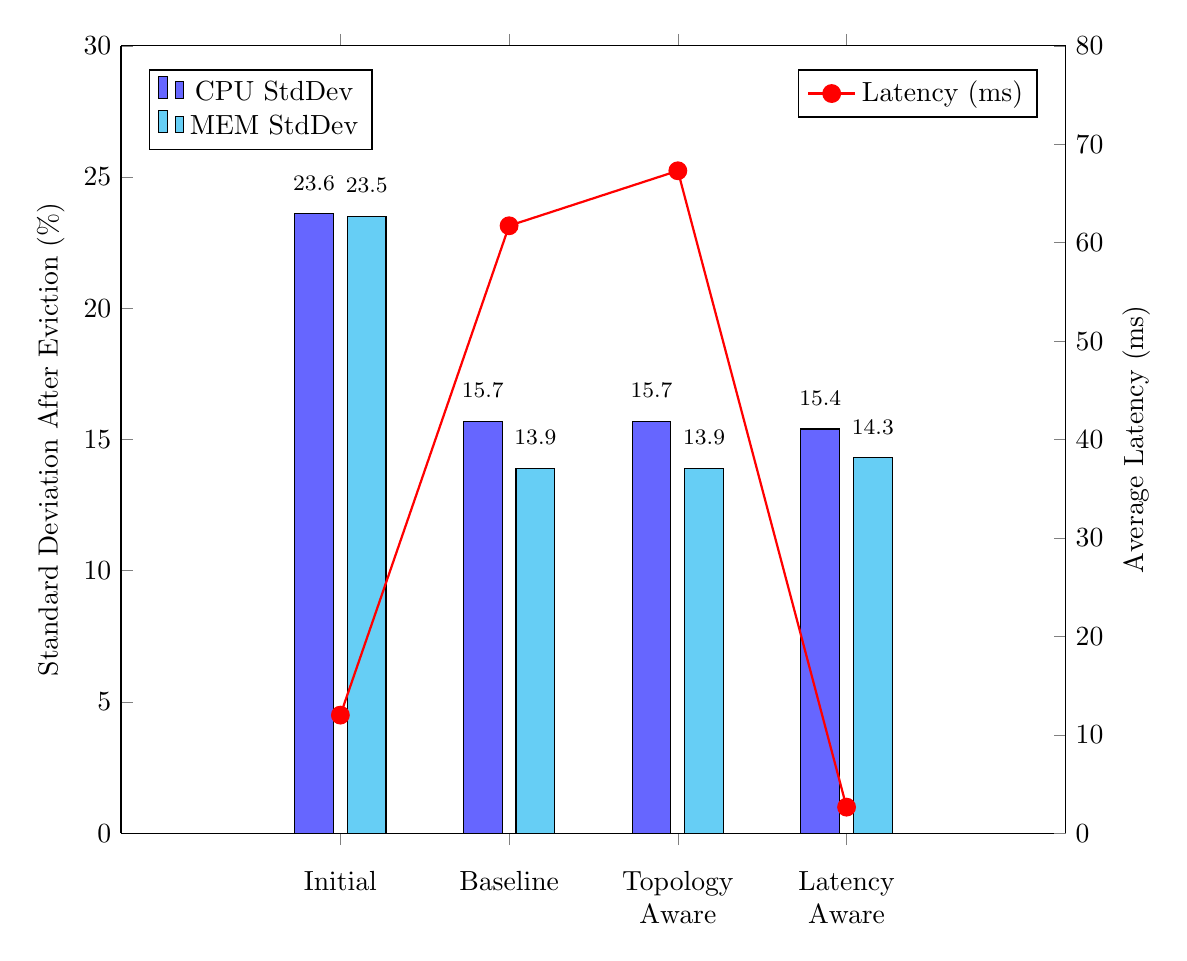
\begin{tikzpicture}
        \pgfplotsset{
            width=12cm,
            height=10cm,
            scale only axis,
            xmin=0.5, xmax=4.5,
            xtick={1,2,3,4},
            xticklabels={Initial, Baseline, {Topology\\Aware}, {Latency\\Aware}},
            xticklabel style={align=center, yshift=-2pt},
            enlarge x limits=0.2,
        }
        
        % Left Y-Axis: CPU & MEM Standard Deviation (Grouped Bar Chart)
        \begin{axis}[
            axis y line*=left,
            ymin=0, ymax=30,
            ylabel={Standard Deviation After Eviction (\%)},
            ylabel near ticks,
            ybar=5pt,
            bar width=14pt,
            legend pos=north west,
            nodes near coords,
            every node near coord/.append style={yshift=5pt, font=\footnotesize},
        ]
            \addplot[fill=blue!60, draw=black] coordinates {
                (1, 23.6)
                (2, 15.7)
                (3, 15.7)
                (4, 15.4)
            };
            \addplot[fill=cyan!60, draw=black] coordinates {
                (1, 23.5)
                (2, 13.9)
                (3, 13.9)
                (4, 14.3)
            };
            \addlegendentry{CPU StdDev}
            \addlegendentry{MEM StdDev}
        \end{axis}

        % Right Y-Axis: Average Latency (Line Chart)
        \begin{axis}[
            axis y line*=right,
            axis x line=none,
            ymin=0, ymax=80,
            ylabel={Average Latency (ms)},
            ylabel near ticks,
            yticklabel pos=right,
            legend pos=north east,
            mark=*,
            mark options={scale=1.5},
        ]
            \addplot[color=red, thick, mark=*] coordinates {
                (1, 12.0)
                (2, 61.717)
                (3, 67.305)
                (4, 2.649)
            };
            \addlegendentry{Latency (ms)}
        \end{axis}
    \end{tikzpicture}
    \caption{Cluster Balance vs. Network Performance.}
    \label{fig:balance_vs_latency}
\end{figure}

The baseline and topology-aware strategies successfully balanced the cluster but caused a catastrophic increase in average latency (spiking from $\sim$4ms to over 60ms). In contrast, the latency-aware strategies (a5-a7) achieved near equal cluster balance while maintaining the latency ($\sim$3ms).

The massive latency spikes observed in the topology-aware tests are primarily caused by the topology model's inability to detect actual network degradation. As visualized in Figure \ref{fig:topology_flaw}, the topology model only evaluates physical zone boundaries (e.g., Cross-Zone to Cross-Zone) and assumes all links are perfectly healthy, it considered degraded nodes as healthy one, resulting on lower or equal network cost calculation. The proposed latency-aware solved this issue by querying Prometheus for real-time metrics, correctly detecting the 160ms degradation and blocking the eviction.

\begin{figure}[H]
    \centering
    \begin{tikzpicture}
        \begin{axis}[
            ybar,
            width=10cm,
            height=6cm,
            ymin=0, ymax=1.5,
            ylabel={Sensitive Pods Placed in Degraded Zone},
            symbolic x coords={Baseline, Topology-Aware, Latency-Aware},
            xtick=data,
            nodes near coords,
            every node near coord/.append style={yshift=5pt, font=\small},
        ]
            \addplot[fill=orange!70, draw=black] coordinates {
                (Baseline, 1)
                (Topology-Aware, 1)
                (Latency-Aware, 0)
            };
        \end{axis}
    \end{tikzpicture}
    \caption{Number of sensitive pods placed into a network-degraded zone.}
    \label{fig:topology_flaw}
\end{figure}

%-----------------------------------------------------------------------------%
\subsubsection{Limitations of Pre-Eviction Filtering (L1)}
\label{subsubsec:netaware4_resultanalysis1_limitation}
%-----------------------------------------------------------------------------%

During testing, we also discovered that the global Pre-Eviction filter (L1) is highly sensitive to configuration heuristics. Table \ref{tab:minbetter_impact} compares the performance of the L1 filter under different \textit{MinBetterPercentage} thresholds against the strategy-embedded L2 filter.

\begin{table}[H]
    \centering
    \resizebox{\textwidth}{!}{%
    \begin{tabular}{l c c}
        \toprule
        \textbf{Configuration} & \textbf{Degraded Pods} & \textbf{Avg Latency (ms)} \\
        \midrule
        L1 Pre-Eviction (MinBetter = 50\%) & 1 & 63.696 \\
        L1 Pre-Eviction (MinBetter = 75\%) & 0 & 4.195 \\
        \midrule
        L2 Strategy Filter (No Tuning Req.) & 0 & 3.017 \\
        \bottomrule
    \end{tabular}%
    }
    \caption{Impact of MinBetterPercentage on L1 Pre-Eviction Filters}
    \label{tab:minbetter_impact}
\end{table}

When the L1 filter was configured with a loose threshold (50\%), it evaluated all schedulable nodes in the cluster and determined that 2 out of the 4 available candidate nodes offered equal or better latency. Because this satisfied the 50\% minimum threshold requirement, the L1 filter allowed the eviction. However, when the pod was rescheduled, the \textit{kube-scheduler} utilized its default \textit{LeastAllocated} strategy. Since the degraded node in the cluster was also completely empty, the scheduler simply placed the pod there to balance CPU and memory resources, completely destroying the workload's latency. 

To mitigate this global-filtering flaw, the L1 threshold had to be strictly tuned to 75\%. In contrast, the L2 filter embeds network-awareness directly into the destination-scoring logic. By evaluating only the exact target nodes rather than the entire cluster, L2 successfully filters out irrelevant "decoy" nodes and provides a much tighter safety net in this scenario, protecting the workload without requiring manual heuristic tuning.

%-----------------------------------------------------------------------------%
\subsubsection{No Filler Pods Scenario}
\label{subsubsec:netaware4_resultanalysis1_hardtradeoff}
%-----------------------------------------------------------------------------%
The previous scenario included generic "filler" pods, which provided the descheduler with a safe alternative to balance the node without touching the network sensitive workloads. To rigorously test the descheduler's logic, we executed a variant where the overutilized nodes were populated exclusively only by network-sensitive pods. 

Table \ref{tab:hard_tradeoff_results} presents the evaluation results when no filler pods were available to be sacrificed.
\begin{table}[H]
    \centering
    \resizebox{\textwidth}{!}{%
    \begin{tabular}{l c c c r c}
        \toprule
        \textbf{Scenario} & \textbf{Evicted Pods} & \textbf{CPU StdDev (\%)} & \textbf{MEM StdDev (\%)} &  \textbf{Avg Latency (ms)} & \textbf{Degraded Pods} \\
        \midrule
        Initial State & - & 23.6 & 21.2 & $\sim$4.0 ms & 0 \\
        \midrule
        a1: Baseline & 6 & 13.1 & 13.9 & 69.073 & 2 \\
        a4: Topology L1+L2 & 6 & 13.1 & 13.9 & 61.249 & 2 \\
        a7: Latency L1+L2 & 0 & 23.6 & 21.2 & 5.102 & 0 \\
        \bottomrule
    \end{tabular}%
    }
    \caption{Descheduler Performance: The "Hard Tradeoff" Scenario (No Filler Pods)}
    \label{tab:hard_tradeoff_results}
\end{table}

This scenario forces the descheduler to make a definitive choice between cluster symmetry and network performance. As shown in Table \ref{tab:hard_tradeoff_results}, the Baseline and Topology-Aware strategies blindly prioritized CPU balancing. They evicted 6 critical pods, successfully balancing the cluster by dropping the CPU and Memory Standard Deviation to $\sim$13\%. However, they placed 2 of those sensitive pods directly into the degraded zone, severely degrading the workload's performance (spiking average latency to $\sim$50ms).

In contrast, the Latency-Aware strategies evaluated the critical pods, detected that evicting any of them would subject them to degraded network conditions, and strictly blocked all evictions (0 Evicted Pods). By intentionally refusing to evict, the Latency-Aware descheduler chose to leave the cluster imbalanced (StdDev remained at $\sim$21-23\%) to guarantee the network integrity of the application. This conclusively proves that the proposed implementation strictly prioritizes application latency over infrastructure symmetry.

\begin{figure}[H]
    \centering
    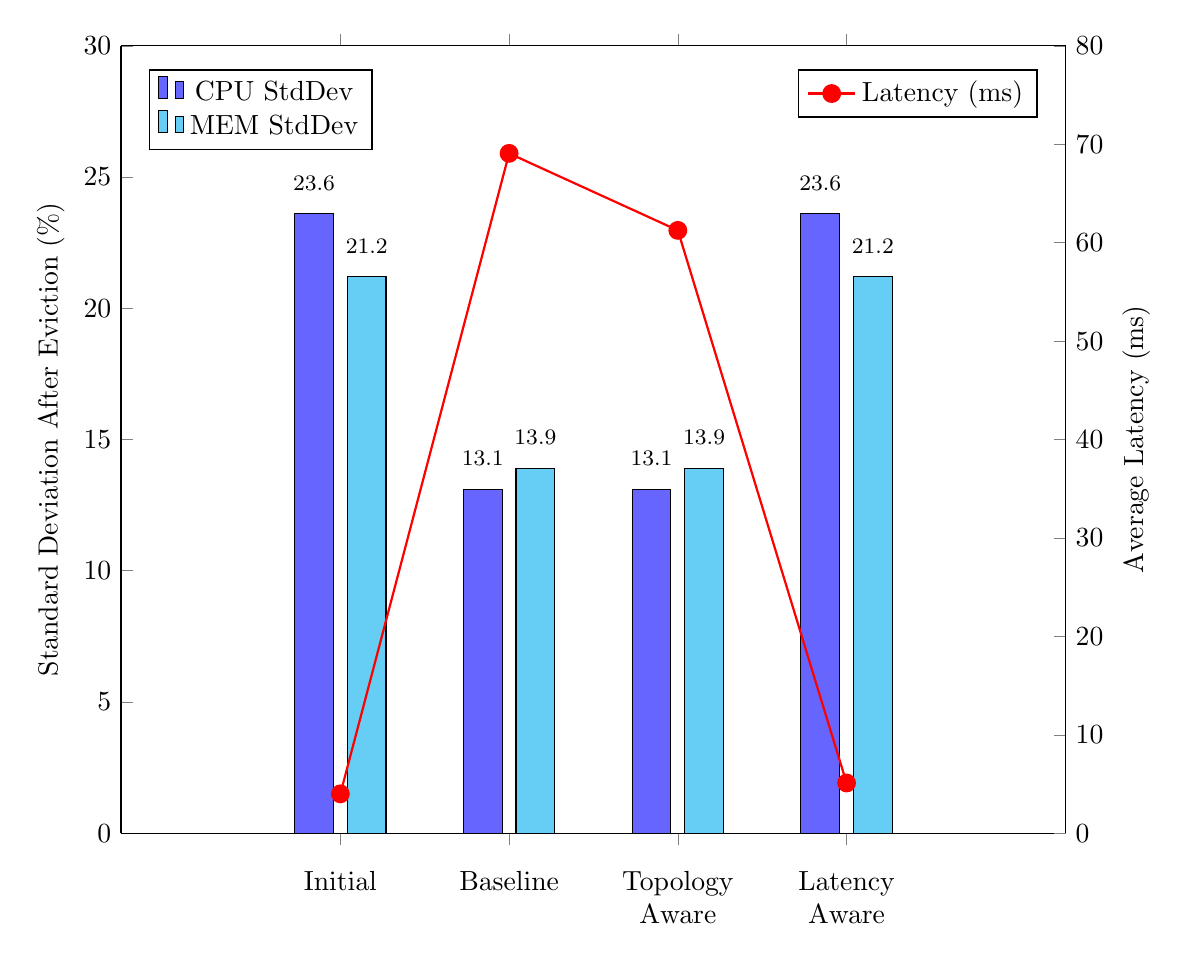
\begin{tikzpicture}
        \pgfplotsset{
            width=12cm,
            height=10cm,
            scale only axis,
            xmin=0.5, xmax=4.5,
            xtick={1,2,3,4},
            xticklabels={Initial, Baseline, {Topology\\Aware}, {Latency\\Aware}},
            xticklabel style={align=center, yshift=-2pt},
            enlarge x limits=0.2,
        }

        \begin{axis}[
            axis y line*=left,
            ymin=0, ymax=30,
            ylabel={Standard Deviation After Eviction (\%)},
            ylabel near ticks,
            ybar=5pt,
            bar width=14pt,
            legend pos=north west,
            nodes near coords,
            every node near coord/.append style={yshift=5pt, font=\footnotesize},
        ]
            \addplot[fill=blue!60, draw=black] coordinates {
                (1, 23.6)
                (2, 13.1)
                (3, 13.1)
                (4, 23.6)
            };
            \addplot[fill=cyan!60, draw=black] coordinates {
                (1, 21.2)
                (2, 13.9)
                (3, 13.9)
                (4, 21.2)
            };
            \addlegendentry{CPU StdDev}
            \addlegendentry{MEM StdDev}
        \end{axis}

        \begin{axis}[
            axis y line*=right,
            axis x line=none,
            ymin=0, ymax=80,
            ylabel={Average Latency (ms)},
            ylabel near ticks,
            yticklabel pos=right,
            legend pos=north east,
            mark=*,
            mark options={scale=1.5},
        ]
            \addplot[color=red, thick, mark=*] coordinates {
                (1, 4.0)
                (2, 69.073)
                (3, 61.249)
                (4, 5.102)
            };
            \addlegendentry{Latency (ms)}
        \end{axis}
    \end{tikzpicture}
    \caption{Cluster Balance vs. Network Performance (No Filler Pods Scenario).}
    \label{fig:hard_tradeoff_latency}
\end{figure}


%-----------------------------------------------------------------------------%
\subsection{Experimental Results: HighNodeUtilization Scenario}
\label{subsec:netaware4_resultanalysis2}
%-----------------------------------------------------------------------------%
\textit{HighNodeUtilization} scenario presents a unique challenge for the descheduler. Unlike \textit{LowNodeUtilization}, which spreads pods across the cluster, \textit{HighNodeUtilization} seeks to pack workloads by evicting pods from underutilized nodes and packing them onto overutilized ones. This relies heavily on the \textit{kube-scheduler}'s \textit{MostAllocated} scoring strategy, which creates a centered gravity to heavy load nodes when scheduling pod.

Table \ref{tab:highnode_results} presents the raw performance of the descheduler when utilizing the strict (\textbf{MinBetterPercentage = 75\%}).
\begin{table}[H]
    \centering
    \resizebox{\textwidth}{!}{%
    \begin{tabular}{l c c c c r c}
        \toprule
        \textbf{Scenario} & \textbf{Evicted Pods} & \textbf{CPU StdDev (\%)} & \textbf{MEM StdDev (\%)} & \textbf{Active Nodes} & \textbf{Avg Latency} & \textbf{Degraded Pods} \\
        \midrule
        Initial State & - & 13.4 & 11.2 & 5 & $\sim$3.0 ms & 0 \\
        \midrule
        b1: Baseline (No Net-Aware) & 4 & 22.1 & 13.8 & 3 & 126.282 ms & 2 \\
        b2: Topology L1 & 4 & 22.1 & 13.8 & 3 & 123.050 ms & 2 \\
        b3: Topology L2 & 4 & 22.1 & 13.8 & 3 & 126.403 ms & 2 \\
        b4: Topology L1+L2 & 4 & 22.1 & 13.8 & 3 & 129.800 ms & 2 \\
        b5: Latency L1 & 2 & 17.7 & 12.5 & 5 & 2.728 ms & 0 \\
        b6: Latency L2 & 2 & 17.7 & 12.5 & 5 & 2.676 ms & 0 \\
        b7: Latency L1+L2  & 2 & 17.7 & 12.5 & 5 & 3.061 ms & 0 \\
        \bottomrule
    \end{tabular}%
    }
    \caption{Descheduler Performance: HighNodeUtilization Scenario}
    \label{tab:highnode_results}
\end{table}

As we observe in Table \ref{tab:highnode_results}, the Baseline and Topology-Aware strategies successfully packed the cluster. By bin-packing the pods, they successfully emptied 2 machines (reducing active nodes from 5 to 3), which naturally caused the CPU and Memory Standard Deviations to increase. However, to achieve this node reclamation, they blindly placed 2 sensitive pods into the degraded zone, causing latency to spike to $\sim$130ms. In contrast, the Latency-Aware strategies successfully blocked the dangerous evictions. While this meant the cluster could not be fully packed (leaving 5 active nodes), it perfectly preserved the $\sim$3ms latency.

\subsubsection{MinBetterCandidatePercent Threshold Tuning for Stricter Evaluation}
\label{subsubsec:netaware4_resultanalysis2_tuning}

Because the descheduler cannot guarantee final placement, it must assess the statistical risk of the \textit{kube-scheduler}'s behavior. We best demonstrate the necessity of the strict 75\% threshold by analyzing the catastrophic failure of the Latency-Aware L2 filter when configured with a looser 50\% threshold.

\begin{figure}[H]
    \centering
    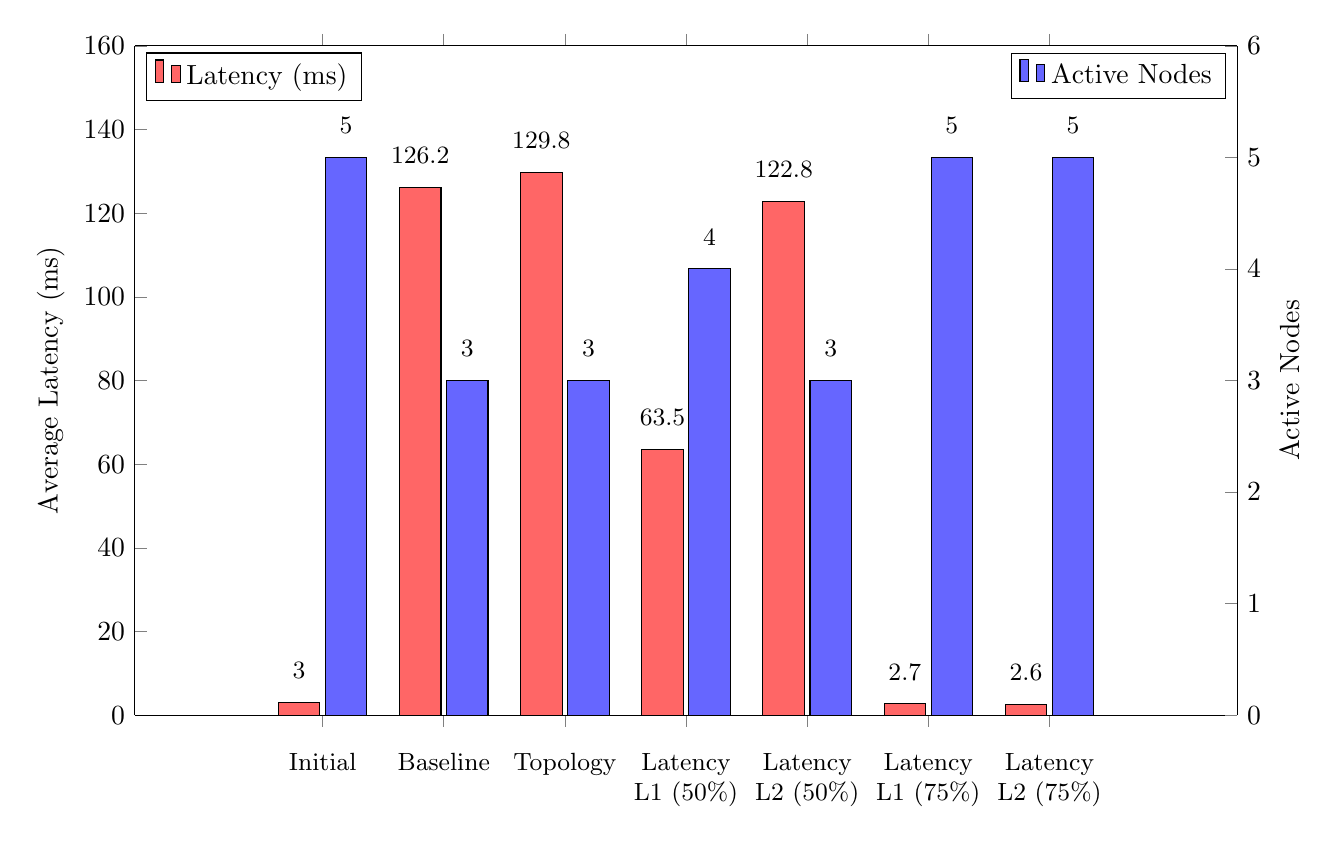
\begin{tikzpicture}
        % Left Y-Axis: Average Latency (Primary Axis)
        \begin{axis}[
            width=14cm,
            height=8.5cm,
            scale only axis,
            ymin=0, ymax=160,
            ylabel={Average Latency (ms)},
            ylabel near ticks,
            ybar,
            bar width=15pt,
            bar shift=-8.5pt, 
            xmin=0.5, xmax=7.5,
            xtick={1,2,3,4,5,6,7},
            xticklabels={
                Initial,
                Baseline, 
                Topology, 
                {Latency\\L1 (50\%)}, 
                {Latency\\L2 (50\%)}, 
                {Latency\\L1 (75\%)}, 
                {Latency\\L2 (75\%)}
            },
            xticklabel style={align=center, font=\small, yshift=-2pt},
            axis y line*=left,
            nodes near coords,
            every node near coord/.append style={yshift=5pt, font=\small},
            legend style={at={(0.01,0.99)}, anchor=north west},
        ]
            \addplot[fill=red!60, draw=black] coordinates {
                (1, 3.0)
                (2, 126.2)
                (3, 129.8)
                (4, 63.5)
                (5, 122.8)
                (6, 2.7)
                (7, 2.6)
            };
            \addlegendentry{Latency (ms)}
        \end{axis}

        % Right Y-Axis: Active Nodes (Secondary Axis)
        \begin{axis}[
            width=14cm,
            height=8.5cm,
            scale only axis,
            ymin=0, ymax=6,
            ytick={0,1,2,3,4,5,6}, 
            ylabel={Active Nodes},
            ylabel near ticks,
            yticklabel pos=right,
            ybar,
            bar width=15pt,
            bar shift=8.5pt,
            xmin=0.5, xmax=7.5,
            axis y line*=right,
            axis x line=none, 
            nodes near coords,
            every node near coord/.append style={yshift=5pt, font=\small},
            legend style={at={(0.99,0.99)}, anchor=north east},
        ]
            \addplot[fill=blue!60, draw=black] coordinates {
                (1, 5)
                (2, 3)
                (3, 3)
                (4, 4)
                (5, 3)
                (6, 5)
                (7, 5)
            };
            \addlegendentry{Active Nodes}
        \end{axis}
    \end{tikzpicture}
    \caption{Performance comparison of \textit{MinBetterCandidatePercent} Tuning}
    \label{fig:highnode_results}
\end{figure}

As shown in Table \ref{tab:highnode_results}, both the L1 and L2 latency filters failed when configured with a loose 50\% threshold. When evaluating the L1 Pre-Eviction filter, it scanned 4 potential candidate nodes and found that 2 of them (worker-2 and worker-3) offered equal or better latency. Because this mathematically satisfied the 50\% threshold, L1 authorized the evictions. However, the \textit{kube-scheduler} subsequently placed one of the sensitive pods into the degraded zone, causing average latency to spike to $\sim$63ms.

Same case happen to latency L2 filter at 50\% that had $\sim$122ms latency spike matching the spike in baseline and topology filter. This occurred due to an architectural boundary between the descheduler and the \textit{kube-scheduler}. The L2 filter strictly evaluated the three highly-utilized target nodes and found that one of them (worker-3) was healthy (0ms latency). Because 1 out of 3 targets satisfied the loose 50\% minimum threshold, the filter approved the eviction. However, once the pod was returned to the scheduling queue, the \textit{kube-scheduler}'s \textit{MostAllocated} algorithm bypassed the healthy node and packed the pods onto the degraded nodes because they had a higher usage allocation. 

The 75\% threshold completely neutralized this threat for both filters, creating a need for minimum 3 and 2 better candidates node for L1 and L2 sequentially. When the L1 filter evaluated the entire cluster under the 75\% configuration, it found that only 2 out of 4 of the scheduleable nodes were safe, immediately blocking the eviction. Similarly, when the L2 filter re-evaluated its specific overutilized target nodes, it recognized that only 1 out of 3 of the available destinations were network-safe. Falling far short of the strict 75\% safety requirement, both filters successfully blocked the network sensitive pods from being evicted.

However, this network protection came as a direct tradeoff for cluster bin-packing efficiency. As illustrated by the "Active Nodes" metric in Figure \ref{fig:highnode_results}, the descheduler's refusal to evict the critical pods meant that the cluster could not be fully packed. While the Baseline strategy successfully emptied 2 machines to save infrastructure resources by reducing active nodes to 3, the Latency-Aware strategies were forced to leave all 5 nodes active to maintain the network latency. This tradeoff proves that our network aware descheduler explicitly prioritizing application health over infrastructure cost savings when a safe placement path cannot be mathematically guaranteed.

%-----------------------------------------------------------------------------%
\subsection{Experimental Results: ResourceDefragmentation Scenario}
\label{subsec:netaware4_resultanalysis3}
%-----------------------------------------------------------------------------%
The \textit{ResourceDefragmentation} scenario evaluates the descheduler's ability to correct multi-dimensional resource skew (CPU vs. Memory) without relying on strict utilization thresholds. This plugin uses the Resource Defragmentation algorithm to specifically target pods whose eviction will mathematically unlock trapped capacity on skewed nodes. 

Because this algorithm optimizes for the geometric "shape" of resource utilization rather than global absolute spread, we evaluate its performance using the \textbf{Mean Absolute Resource Imbalance Index (RII)}. RII is defined as the absolute difference between a node's CPU utilization percentage and its Memory utilization percentage ($|CPU\% - MEM\%|$). A lower Mean Absolute RII indicates a better balanced, symmetrical cluster.

Prior to the descheduler execution, the cluster was forced into a highly fragmented state (Mean Absolute RII: \textbf{50.7\%}), with nodes exhibiting massive orthogonal skews (e.g., 90\% CPU vs 51\% Mem, and 10\% CPU vs 82\% Mem).

Table \ref{tab:resourcedefrag_results} presents the raw performance of the descheduler across the three filtering strategies.
\begin{table}[htbp]
    \centering
    \resizebox{\textwidth}{!}{%
    \begin{tabular}{l c c r c}
        \toprule
        \textbf{Scenario} & \textbf{Evictions} & \textbf{Mean Absolute RII (\%)} & \textbf{Avg Latency} & \textbf{Degraded Pods} \\
        \midrule
        Initial State & - & 50.7\% & $\sim$8.0 ms & 0 \\
        \midrule
        r1: Baseline & 8 & 19.9\% & 167.216 ms & 2 \\
        r2: Topology L1 & 8 & 19.9\% & 165.783 ms & 2 \\
        r3: Latency L1 & 8 & 17.9\% & 8.762 ms & 0 \\
        \bottomrule
    \end{tabular}%
    }
    \caption{Descheduler Performance: ResourceDefragmentation Scenario}
    \label{tab:resourcedefrag_results}
\end{table}

As shown in Table \ref{tab:resourcedefrag_results}, the baseline \textit{ResourceDefragmentation} plugin successfully identified the orthogonal CPU and Memory skews within the cluster and executed 8 evictions to aggressively balance the nodes (reducing the Mean Absolute RII from 50.7\% down to 19.9\%). However, because the Resource Defragmentation algorithm strictly optimizes for mathematical resource symmetry, it eagerly selected the network-sensitive \textit{payment} pods for eviction, predicting that moving them to the memory-heavy degraded nodes would perfectly resolve the cluster's resource skew. Consequently, the baseline strategy placed 2 critical pods directly into the network-degraded zone, causing a catastrophic latency spike to $\sim$167ms. 

The Topology-Aware L1 filter failed to prevent this. Because the topology model relies on static physical boundaries, it was entirely blind to the active network degradation. It approved the eviction of the critical pods, resulting in the exact same mathematical resource balance and the exact same network latency violation ($\sim$165ms) as the baseline. 

Our proposed Latency-Aware L1 filter achieved a much better outcome: it successfully preserved the application's network latency while simultaneously allowing the descheduler to fix the cluster's resource fragmentation. When the Resource Defragmentation algorithm initially selected the sensitive \textit{payment} pods for eviction, our Latency-Aware filter queried the real-time Prometheus metrics, detected the massive degradation on the target nodes, and strictly blocked the eviction. 

Because the Kube-Descheduler framework operates iteratively, blocking the \textit{payment} pods forced the Resource Defragmentation algorithm to evaluate the next-best candidates: the generic \textit{filler-cpu} pods. Because these filler pods were not part of the sensitive network group, our filter safely allowed their eviction. By actively steering the descheduler away from the critical workloads, we forced the cluster to resolve its resource fragmentation using expendable pods. This resulted in an even better reduction in resource skew (Mean RII dropped to 17.9\%) while completely protecting the network integrity of the application (0 degraded pods, $\sim$8ms latency). 

\subsubsection{Defragmentation Performance and Network Latency Trade-offs}
\label{subsubsec:netaware4_resultanalysis3_tradeoff}

Figure \ref{fig:resourcedefrag_latency} visually summarizes the performance of the three filtering strategies, highlighting our Latency-Aware plugin's ability to decouple cluster resource balancing from network performance degradation.
\begin{figure}[htbp]
    \centering
    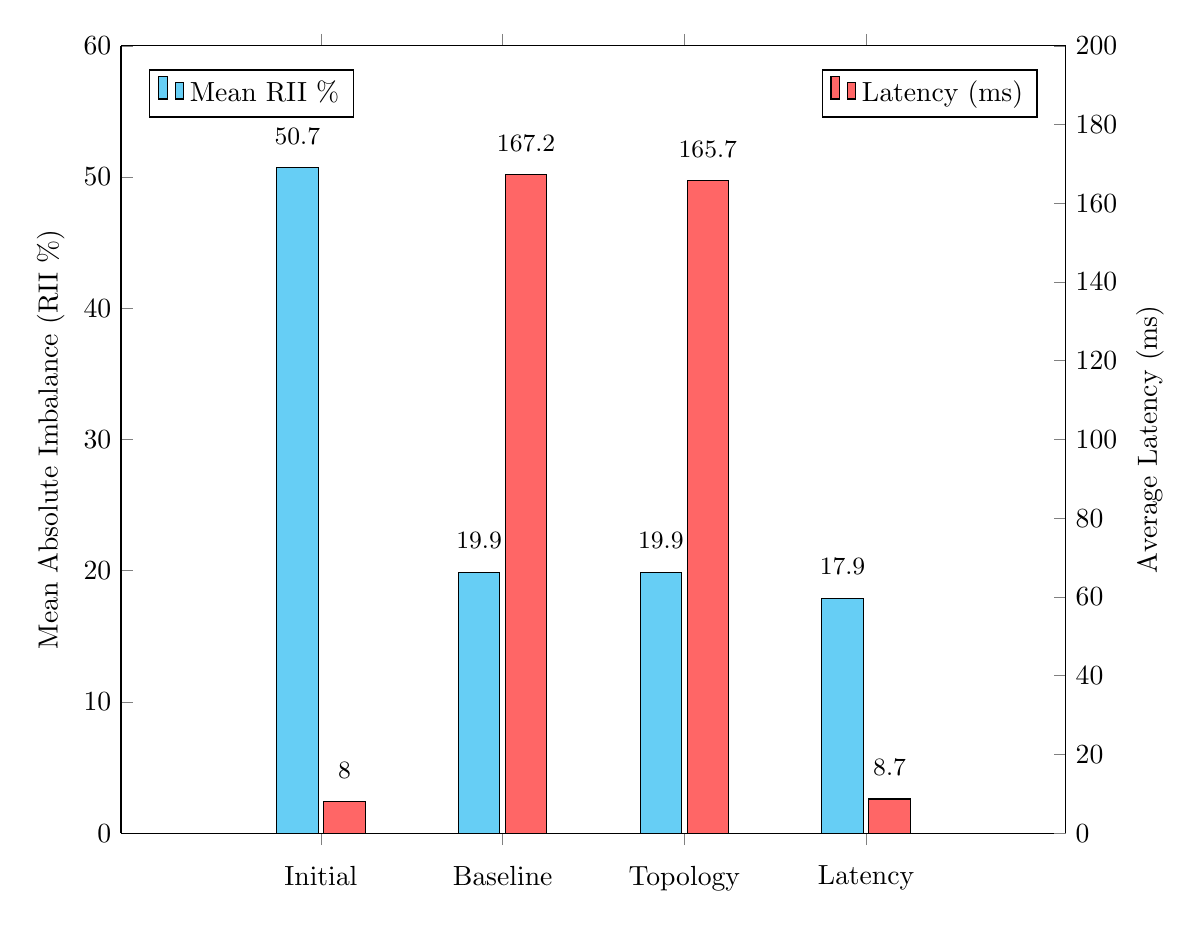
\begin{tikzpicture}
        \pgfplotsset{
            width=12cm,
            height=10cm,
            scale only axis,
            xmin=0.5, xmax=4.5,
            xtick={1,2,3,4},
            xticklabels={Initial, Baseline, Topology, Latency},
            enlarge x limits=0.15,
        }
        
        % Left Y-Axis: Mean Absolute RII
        \begin{axis}[
            axis y line*=left,
            ymin=0, ymax=60,
            ylabel={Mean Absolute Imbalance (RII \%)},
            ybar,
            bar width=15pt,
            bar shift=-8.5pt,
            legend pos=north west,
            nodes near coords,
            every node near coord/.append style={yshift=5pt, font=\small},
        ]
            \addplot[fill=cyan!60, draw=black] coordinates {
                (1, 50.7)
                (2, 19.9)
                (3, 19.9)
                (4, 17.9)
            };
            \addlegendentry{Mean RII \%}
        \end{axis}
        % Right Y-Axis: Average Latency (Bar Chart)
        \begin{axis}[
            axis y line*=right,
            axis x line=none,
            ymin=0, ymax=200,
            ylabel={Average Latency (ms)},
            ylabel near ticks,
            yticklabel pos=right,
            ybar,
            bar width=15pt,
            bar shift=8.5pt,
            nodes near coords,
            every node near coord/.append style={yshift=5pt, font=\small},
            legend pos=north east,
        ]
            \addplot[fill=red!60, draw=black] coordinates {
                (1, 8.0)
                (2, 167.2)
                (3, 165.7)
                (4, 8.7)
            };
            \addlegendentry{Latency (ms)}
        \end{axis}
    \end{tikzpicture}
    \caption{Mean Absolute Resource Imbalance (RII) vs. Network Performance.}
    \label{fig:resourcedefrag_latency}
\end{figure}

The results from the Resource Defragmentation scenario mathematically prove that our Latency-Aware plugin does not inherently compromise the core goal of the defragmentation algorithm. Instead of blindly moving critical workloads to satisfy a mathematical equation, the plugin intelligently evaluates network safety and blocks evictions that violate it. As demonstrated by the 17.9\% final RII, the presence of these expendable pods allowed the steered approach to achieve a slightly superior geometric resource balance compared to the baseline. However, as established in our earlier Hard Tradeoff experiments, if no such filler pods were available, the Latency-Aware plugin would actively choose to leave the cluster in a fragmented state (higher Mean RII) to guarantee network integrity like showed in \ref{tab:hard_tradeoff_results}
